
\documentclass[crop, tikz, border=0pt]{standalone}
\usetikzlibrary{matrix}
\usetikzlibrary{patterns}
\usepackage{varwidth}
\usepackage{amsmath}
\usepackage{amssymb}
\usepackage{color}

\begin{document}
\color{white}
\definecolor{red}{HTML}{fd5000}
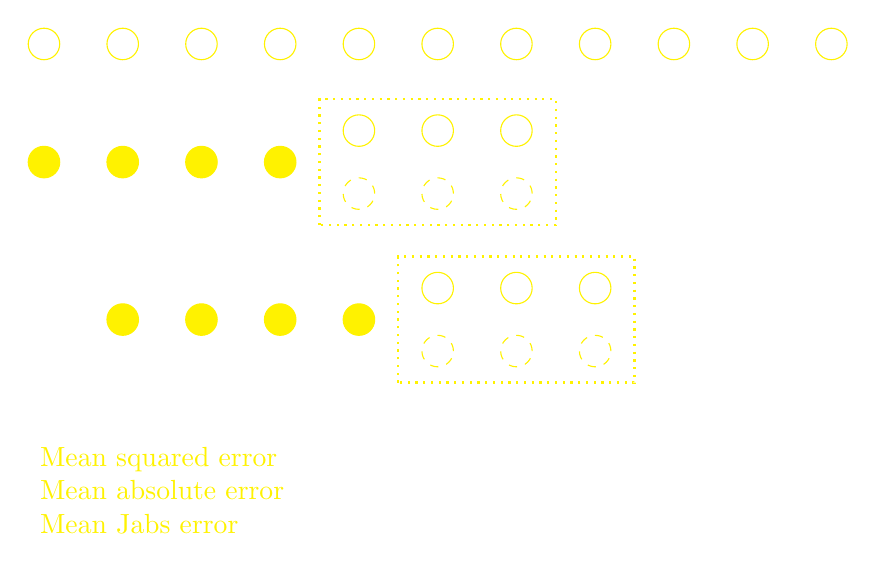
\begin{tikzpicture}[draw=yellow]
%\tikzset{rectangle node/.style = {rectangle, inner sep=1pt, draw, fill=white}}
\tikzset{edge/.style = {->,> = latex, line width=.5 pt}}

   
\foreach \x in {0, 1, 2, 3, 4, 5, 6, 7, 8, 9, 10}
   {\draw (\x, .5) circle (.2);}

\foreach \x in {0, 1, 2, 3}
  {\draw [fill=yellow] (\x, -1) circle (.2);}

\foreach \x in {4, 5, 6}
{\draw [dashed] (\x, -1.4) circle (.2);}


\foreach \x in {4, 5, 6}
{\draw  (\x, -.6) circle (.2);}

\draw[thick, dotted] (3.5, - 1.8) rectangle ++ (3, 1.6);

\foreach \x in {1, 2, 3, 4}
{\draw [fill=yellow] (\x, -3) circle (.2);}

\foreach \x in {5, 6, 7}
{\draw [dashed] (\x, -3.4) circle (.2);}


\foreach \x in {5, 6, 7}
{\draw  (\x, -2.6) circle (.2);}

\draw[thick,dotted]     (4.5, - 3.8) rectangle ++ (3, 1.6);

 \node[below, color=yellow, align=left] at (1.5, -4.5) {
 Mean squared error \\ 
 Mean absolute error \\ 
 Mean Jabs error
}; 
    
\end{tikzpicture}
\end{document}